\bookchapter{Balance and the centre of mass}\label{ch:ctl2}

\section*{Explanation}
A soccer robot walks, kicks, gets pushed by another robot and stands up again. All of this depends on one question: \emph{does the robot stay on its feet?} This chapter gives the simple physics that answers it. The ideas (centre of mass, support polygon, the inverted pendulum, the capture point) are used in every walking controller, from the hand-written ones to the learned policies of the K1 chapters, where the same quantities appear in the observations and in the reward.

\section*{The centre of mass}
A robot consists of many parts: feet, legs, a trunk, a head, batteries. For the question of balance they can all be replaced by one point, the \textbf{centre of mass} (CoM): the average of the positions of the parts, \emph{weighted by their masses}. For parts with masses $m_i$ at positions $(x_i,z_i)$ (here $x$ is horizontal and $z$ is height):
\[
x_{\text{CoM}}=\frac{\sum_i m_i x_i}{\sum_i m_i},\qquad z_{\text{CoM}}=\frac{\sum_i m_i z_i}{\sum_i m_i}.
\]
It is the point where the gravity of the whole robot seems to pull, and the point that moves like a single mass when forces act on the robot.

\begin{example}
A simplified robot has three parts: legs ($5$\,kg, at $x=0$, $z=0.30$\,m), trunk ($3$\,kg, at $x=0.10$, $z=0.55$) and a head with an arm stretched backwards ($2$\,kg, at $x=-0.05$, $z=0.80$). The total mass is $10$\,kg, and
\[
x_{\text{CoM}}=\frac{5\cdot0+3\cdot0.10+2\cdot(-0.05)}{10}=0.02\,\text{m},\quad
z_{\text{CoM}}=\frac{5\cdot0.30+3\cdot0.55+2\cdot0.80}{10}=0.475\,\text{m}.
\]
The CoM is $2$\,cm in front of the legs and $47.5$\,cm above the ground. If the trunk bends forward, $x_{\text{CoM}}$ grows without any foot moving: that is how a robot (or you) shifts its weight.
\end{example}

\section*{Static balance: the support polygon}
Standing still, the robot touches the ground only with the soles of its feet. The smallest convex area that contains all contact surfaces (think of a rubber band around both feet) is the \textbf{support polygon}. A robot at rest does not fall as long as the vertical projection of the CoM onto the ground lies \emph{inside} the support polygon. With both feet on the ground the polygon is large, standing on one foot it is only the sole.

\begin{center}
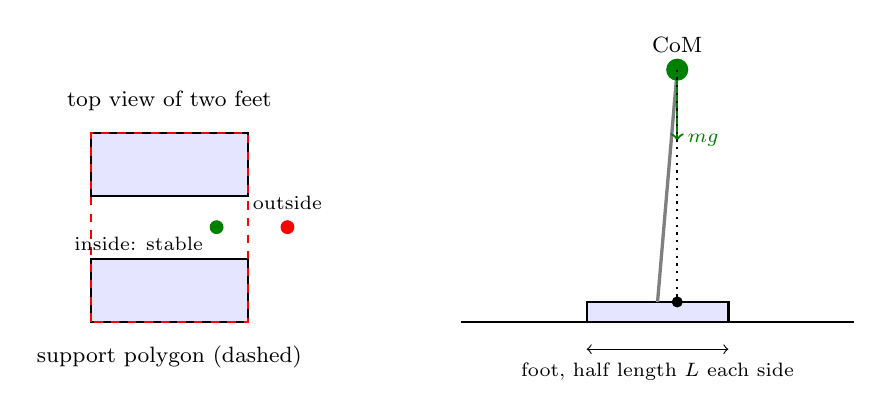
\begin{tikzpicture}[scale=1.0]
 % ground view (top)
 \draw[fill=blue!10,thick] (0,0) rectangle (2,0.8);
 \draw[fill=blue!10,thick] (0,1.6) rectangle (2,2.4);
 \draw[thick,dashed,red] (0,0) rectangle (2,2.4);
 \fill[green!50!black] (1.6,1.2) circle (2.5pt); \node[font=\scriptsize,below left] at (1.55,1.2) {inside: stable};
 \fill[red] (2.5,1.2) circle (2.5pt); \node[font=\scriptsize,above] at (2.5,1.3) {outside};
 \node[font=\footnotesize] at (1,-0.45) {support polygon (dashed)};
 \node[font=\footnotesize] at (1,2.8) {top view of two feet};
 % side view
 \begin{scope}[xshift=7.2cm]
 \draw[thick] (-2.5,0)--(2.5,0);
 \draw[fill=blue!10,thick] (-0.9,0) rectangle (0.9,0.25);
 \draw[very thick,gray] (0,0.25)--(0.25,3.2);
 \fill[green!50!black] (0.25,3.2) circle (4pt); \node[font=\footnotesize,above] at (0.25,3.3) {CoM};
 \draw[->,thick,green!50!black] (0.25,3.2)--(0.25,2.3) node[right,font=\scriptsize]{$m g$};
 \draw[dotted,thick] (0.25,3.2)--(0.25,0.25); \fill[black] (0.25,0.25) circle (2pt);
 \draw[<->] (-0.9,-0.35)--(0.9,-0.35); \node[font=\scriptsize,below] at (0,-0.4) {foot, half length $L$ each side};
 \end{scope}
\end{tikzpicture}
\captionof{figure}{Left: top view of two feet and the support polygon. Right: side view (not to scale). The CoM is above the foot, so the robot stands.}
\end{center}

\section*{Dynamic balance: the inverted pendulum}
A walking robot is \emph{not} in static balance: during each step the CoM is outside the sole of the single foot that touches the ground, and the robot is, for a moment, falling. The simplest model that captures this is the \textbf{linear inverted pendulum}: all the mass is in the CoM at a constant height $h$, held by a massless leg that touches the ground at the point $p$. Here $p$ is the point where the ground force acts (the \textbf{centre of pressure}); it can be moved inside the sole, by shifting the pressure between heel and toe, or by pushing with the ankle.

Take the torques around $p$. Gravity pulls with $mg$ at the horizontal distance $x-p$ and tends to tip the robot over; the horizontal acceleration $a=\ddot x$ of the CoM at the height $h$ gives the torque $m\,a\,h$ in the other direction. For the balance of torques:
\[
m g\,(x-p)=m\,\ddot x\,h\quad\Longrightarrow\quad \ddot x=\frac{g}{h}\,(x-p)=\frac{x-p}{T_c^{2}},\qquad T_c=\sqrt{\frac{h}{g}} .
\]
The number $T_c$ is the time constant of the fall. If the CoM is displaced from $p$, it is accelerated \emph{away} from $p$, with an acceleration proportional to the displacement: the equation of a repulsive spring. With $p=0$ and $x(0)=x_0$, $\dot x(0)=0$ the solution is $x(t)=x_0\cosh(t/T_c)$, which grows exponentially, by a factor $e\approx2.7$ for each $T_c$ (roughly each $T_c\cdot 0.9$ the distance doubles).

\begin{example}
A robot with the CoM at the height $h=0.5$\,m has $T_c=\sqrt{0.5/9.81}=0.226$\,s. It stands with the CoM $x_0=1$\,cm in front of the support point $p=0$ and nobody corrects it. After $0.2$\,s the CoM is $1.4$\,cm away, after $0.5$\,s $4.6$\,cm, after $1.0$\,s $41.5$\,cm: the fall is slow at the beginning and then sudden. The CoM is $25$\,cm away after $0.89$\,s.
\end{example}

\begin{center}
\begin{tikzpicture}
\begin{axis}[width=0.8\linewidth,height=5cm,xlabel={time $t$ (s)},ylabel={CoM displacement (cm)},xmin=0,xmax=1,ymin=0,ymax=45,grid=both]
 \addplot[red,thick] table[x=t,y=x] {chapters/part09_control_perception/02_balance_and_centre_of_mass/fall.dat};
\end{axis}
\end{tikzpicture}
\captionof{figure}{An uncontrolled inverted pendulum ($h=0.5$\,m) that starts $1$\,cm from its support point. After a slow start the displacement grows exponentially. The model is valid only while the angle is small; later the real robot has fallen.}
\end{center}

\section*{Balancing means moving the support point}
The equation shows what the controller can do: it cannot change gravity, but it \emph{can choose $p$}. If $p$ is moved to the same side as the CoM, the acceleration turns back. Choosing $p=x$ gives $\ddot x=0$. The limits are the sole: $|p|\le L$, where $L$ is the half length of the foot. This is called the \textbf{ankle strategy}. If it is not enough the robot must take a step (the \textbf{stepping strategy}), which moves the whole support polygon.

\subsection*{The capture point}
When can the ankle strategy still save the robot? Look at the quantity
\[
\xi=x+T_c\,\dot x ,
\]
the \textbf{capture point}: the position of the CoM plus the speed times $T_c$. From the equation of motion one finds $\dot\xi=(\xi-p)/T_c$. If $p=\xi$ then $\dot\xi=0$, and, because $\xi=x+T_c\dot x$ is constant, the CoM stops, with $\dot x\to 0$ and $x\to\xi$: the robot comes to rest above the point $\xi$. This can be done by the ankle strategy exactly when the capture point lies inside the foot, $|\xi|\le L$; and if $|\xi|>L$ then $\xi$ grows without limit for every $p$ in the foot, and the robot falls unless it steps. Therefore the capture point is the best single number for ``is this robot in trouble?''.

\begin{example}
$h=0.5$\,m, so $T_c=0.226$\,s; foot half length $L=5$\,cm. A push gives the CoM, which started above the ankle ($x=0$), the speed $v_0$. The capture point is $\xi=T_cv_0$ and the limit is $v_0\le L/T_c=0.05/0.226=0.22$\,m/s. A push of $0.20$\,m/s can be absorbed by the ankles alone ($\xi=4.5$\,cm), a push of $0.24$\,m/s cannot ($\xi=5.4$\,cm).
\end{example}

\begin{center}
\begin{tikzpicture}
\begin{axis}[width=0.8\linewidth,height=5.5cm,xlabel={time $t$ (s)},ylabel={CoM position (cm)},xmin=0,xmax=1.5,ymin=-1,ymax=12,grid=both,legend pos=north east,legend style={font=\footnotesize}]
 \addplot[blue,thick] table[x=t,y=a] {chapters/part09_control_perception/02_balance_and_centre_of_mass/push.dat};
 \addplot[green!50!black,thick] table[x=t,y=b] {chapters/part09_control_perception/02_balance_and_centre_of_mass/push.dat};
 \addplot[orange,thick] table[x=t,y=c] {chapters/part09_control_perception/02_balance_and_centre_of_mass/push.dat};
 \addplot[red,thick] table[x=t,y=d] {chapters/part09_control_perception/02_balance_and_centre_of_mass/push.dat};
 \addplot[black,dashed] coordinates {(0,5)(1.5,5)};
 \legend{$0.15$\,m/s,$0.20$\,m/s,$0.22$\,m/s,$0.24$\,m/s,foot edge $L$}
\end{axis}
\end{tikzpicture}
\captionof{figure}{Simulated pushes ($h=0.5$\,m, $L=5$\,cm) that give the CoM the speed in the legend. The ankle controller $p=\operatorname{clamp}(1.5\,\xi,\,-L,\,L)$ stops the three weaker pushes (the last one just barely, after nearly reaching the foot edge); the push of $0.24$\,m/s makes the robot fall.}
\end{center}

\begin{aibox}[Why this matters for learned walking]
A neural network that has learned to walk (Part on reinforcement learning) has found, without being told, behaviour that keeps the capture point close to the feet, with steps that land where it is going. When you design the reward or the observation of a policy, quantities such as the CoM height, its speed and the capture point are good candidates; and they are the numbers that a debug tool should display during a fall.
\end{aibox}

\section*{In code}
The decision ``stand, use the ankles or step?'' is a few lines. We use a safety margin: the ankle strategy is chosen only if the capture point is within $80\%$ of the foot. Numbers are in metres.
%rs:capture
\begin{verbatim}
#[derive(Debug, PartialEq)]
enum Action {
    Ankle,             // enough to shift the pressure under the foot
    Step(f64),         // take a step, with the foot at this position
}

const G: f64 = 9.81;

fn capture_point(x: f64, v: f64, h: f64) -> f64 {
    x + v * (h / G).sqrt()
}

fn decide(x: f64, v: f64, h: f64, half_foot: f64) -> Action {
    let xi = capture_point(x, v, h);
    if xi.abs() <= 0.8 * half_foot {
        Action::Ankle
    } else {
        Action::Step(1.1 * xi)       // a little beyond the capture point
    }
}

fn main() {
    for v in [0.10, 0.15, 0.20, 0.30] {
        let xi = capture_point(0.0, v, 0.5);
        println!("v {v:.2}  xi {xi:.4}  {:?}", decide(0.0, v, 0.5, 0.05));
    }
}
\end{verbatim}
prints, for a CoM that is above the ankle at the moment of the push ($x=0$),
\begin{center}\small\ttfamily
\begin{tabular}{@{}l@{}}
v 0.10  xi 0.0226  Ankle\\
v 0.15  xi 0.0339  Ankle\\
v 0.20  xi 0.0452  Step(0.04966760050843041)\\
v 0.30  xi 0.0677  Step(0.0745014007626456)
\end{tabular}
\end{center}
The push of $0.20$\,m/s could still be absorbed by the ankles (Figure above, $\xi=4.5$\,cm$<5$\,cm), but with the margin of $80\%$ the program already prepares a step: a controller must not plan with the last millimetre of the foot, because the model is not exact and the real sole is not rigid. How far to step, and with which foot, is the subject of the walking chapter of the K1 part (Chapter~\ref{ch:k13}).

\begin{keyidea}[What the model leaves out]
The inverted pendulum has no legs with mass, no swinging arms and no trunk that can turn. A real robot can also change its balance by moving the arms and bending the trunk (it stores \emph{angular momentum}), by pushing against a second contact (a hand on the wall) or by a controlled fall into a roll. The model is a first guide: the numbers $T_c$ and $\xi$ say how much time and how much room you have.
\end{keyidea}

\section*{Practice problems}
\begin{enumerate}[label=\textbf{\thechapter.\arabic*}]
  \item A robot is modelled by two parts: $4$\,kg at $(x,z)=(0,0.20)$ and $1$\,kg at $(0.30,0.60)$ (metres). Compute the centre of mass.
  \item Each foot is a rectangle $0.20$\,m long ($x$ from $-0.10$ to $0.10$) and $0.08$\,m wide; the right foot covers $y\in[0.05,0.13]$, the left foot $y\in[-0.13,-0.05]$. The CoM is projected on the ground at $A=(0.08,0.02)$, $B=(0.12,0)$ and $C=(0,0.14)$. For each point: is it inside the support polygon with both feet on the ground? And with only the right foot?
  \item Compute the time constant $T_c=\sqrt{h/g}$ for $h=0.3$\,m, $0.8$\,m and $1.0$\,m. Which robot has more time to react?
  \item An uncontrolled inverted pendulum ($h=0.5$\,m, $x(t)=x_0\cosh(t/T_c)$) starts $2$\,cm from its support point. After which time is it $20$\,cm away? (Use $\cosh^{-1}10=2.993$.)
  \item $h=0.5$\,m, $L=5$\,cm. The CoM is $2$\,cm in front of the ankle and moves forward at $0.15$\,m/s. Compute the capture point. Can the ankle strategy save the robot? What if the speed is $0.10$\,m/s?
  \item A taller robot ($h=0.8$\,m) has feet with half length $L=8$\,cm. What is the largest speed of the CoM, above the ankle, for which the ankles alone can still stop it?
  \item Compare two robots of the same shape, one with $h=0.5$\,m and $L=5$\,cm, one twice as large ($h=1.0$\,m, $L=10$\,cm). Compute $T_c$ and the largest recoverable push speed $L/T_c$ for both, and explain in words which of the two reacts more slowly and which can absorb the faster push.
  \item The robot has a mass of $10$\,kg and stands with the CoM $3$\,cm in front of the ankle. Which torque must the ankle motor apply to hold the robot still? What is the largest forward offset of the CoM that a motor with a limit of $3$\,N\,m can hold?
  \item Write a Python simulation of the uncontrolled pendulum ($h=0.5$\,m, $x_0=1$\,cm, step $1$\,ms) and find the time at which $x$ reaches $5$\,cm. Compare with $T_c\cosh^{-1}(5)$ (use $\cosh^{-1}5=2.292$).
  \item[\textbf{\thechapter.10}$\star$] Write a Rust program with the ankle controller $p=\operatorname{clamp}(1.5\,\xi,-L,L)$ for $h=0.5$\,m and $L=5$\,cm (step $1$\,ms, $3$ seconds), which reports for a given push speed $v_0$ whether the robot recovers ($|x|$ stays below $0.5$\,m). Find the largest recoverable $v_0$ by bisection and compare with $L/T_c$. Then discuss: with a delay of $50$\,ms in the sensor, would the real limit be larger or smaller, and why?
\end{enumerate}
